\documentclass[12pt]{article}


\usepackage[dvips,letterpaper,margin=0.75in,bottom=0.75in]{geometry}
\usepackage{cite}
\usepackage{slashed}
\usepackage{graphicx}
\usepackage{amsmath}

\usepackage[american,fulldiode,oldvoltagedirection]{circuitikz}
\tikzset{component/.style={draw,thick,circle,fill=white,minimum size =0.75cm,inner sep=0pt}}

\begin{document}
\ctikzset{bipoles/thickness=1}
\ctikzset{bipoles/length=0.6cm}

\title{Planck's Constant} 

\maketitle

\section{Introduction}

In this lab, we will measure Planck's constant by measuring the
$V$-$I$ curves of three different colored light emitting diodes
(LEDs).

An LED is a particular type of diode for which the recombination of
electrons and holes produces photons, typically in the visible light
spectrum.  These diodes have an activation voltage given by:
\begin{equation} \label{eqn:va}
V_{\rm A} = \phi + \frac{hc}{e}\frac{1}{\lambda}
\end{equation}
where $\lambda$ is the wave-length of the light produced by the diode,
and $\phi$ is the contribution to the voltage drop due to other
effects in the $p-n$ junctions.  The diodes we are using have been
chosen to ensure that $\phi$ is approximately constant across all
three diodes.

The quantity
\begin{displaymath}
\frac{hc}{e}
\end{displaymath}
can therefore be determine from the slope of the activation voltage as a function of $1/\lambda$.

The 2018 redefinition of the SI is means that the quantity
\begin{displaymath}
hc = 1.23984193~\rm eV \mu m
\end{displaymath}
is technically now exactly known, because the values $h$, $c$, and $e$
are now taken as exact values which define the corresponding SI
units. Of course, it is still useful and fun to measure this quantity
ourselves in the lab.  We'll interpret this measurement as our
determination of Planck's constant, using the known values for $c$ and
$e$.

\section{Experimental Setup}

To determine the activation voltage of our three LEDs, we'll make measurements as shown in Fig.~\ref{fig:concept_setup}.  By varying the voltage $V_1$ and measuring the current and voltage drop across the diode, we can determine the $V-I$ curve for each diode and accurately determine it's activation voltage.

\begin{figure}[htbp]
\begin{center}
\begin{circuitikz}[line width=1pt]
\draw (0,0) to[voltage source,bipoles/length=1.5cm,l=$V_1$] ++(0,4.0) to[short] ++(2.0,0) coordinate(C);
\draw (C) to[R, l_=$R_1$] ++(0,-2.0) coordinate(B) to[empty led, bipoles/length=1.0cm] ++(0,-2.0) coordinate(A) to[short] ++(-2.0,0.0);
\draw (A) to[short,*-] ++(1.5,0) to[short] ++(0,0.8) node[component]{V} to[short] ++(0,0.8) to[short,-*] ++(-1.5,0);
\draw (C) to[short,*-] ++(1.5,0) to[short] ++(0,-0.8) node[component]{V} to[short] ++(0,-0.8) to[short,-*] ++(-1.5,0);
\end{circuitikz} 
\end{center}
\caption{Conceptual setup for the LED measurements}
\label{fig:concept_setup}
\end{figure}

\begin{figure}[htbp]
\begin{center}
\begin{circuitikz}[line width=1pt]
  \draw (0,0) node[left]{pin $A0$} to[short,o-] ++(1.0,0.0)
  to[american potentiometer,n=mypot,l_=$R_{\rm pot}$] ++(0,-4) to[short,-o] ++(-1.0,0.0) node[left]{pin $A2$}  
  (mypot.wiper) to[short,-*] ++(2.0,0) coordinate(X) to[short,-o] ++(1.0,0)node[right]{pin $A1$};
  \draw (X)  to[resistor,l=$R_{\rm cur}$] ++(0,-2.0) coordinate(X) to[empty led, bipoles/length=1.0cm]  ++(0,-2.0) node[ground,yscale=2.0]{};
  \draw (X) to[short,*-o] ++(1.0,0)node[right]{pin $A4$};
\end{circuitikz} 
\caption{The experimental setup used to measure the V-I response of an LED diode.
}
\label{fig:setup}
\end{center}
\end{figure}

To implement this measurement with your Arduino kit, use the
experimental setup shown in Fig.~\ref{fig:setup}.  By configuring pin
A0 to $5~\rm V$ and A2 as an output pin set to ground, the variable
resistor $R_{\rm pot}$ becomes a potentiometer just as in the LED
dimming example of the introductory lab, with a variable voltage at
pin A1 controlled by turning the knob on your custom shield.  This
variable DC voltage will be applied to the device-under-test (one of
the three LEDs reserved for this lab in the small plastic bag included
with your kit) through the $100~\rm \Omega$ resistor $R_{\rm cur}$
(also reserved in the small plastic bag).  By measuring the voltage at
pin A1 and pin A4, you can calculate the voltage across and current
through the diode.

To setup the aparatus, recall that the potentiometer is already
installed on your custom protoshield.  Use the tiny bread board, small
bits of wire, and components included in your kit.  If we had all
quarter to work together in person, I would have spent as much time as
I could teaching you the one real trick that I know: divide and
conquer.  Here's how I would implement this circuit, broken into
multiple, {\bf testable} steps.

\vskip 1cm
\noindent
{\bf Step 1:} Create a circuit to test the LED and resistor part of
the circuit independent of the potentiometer.  Instead of driving the
LED from A1, drive it from one of the Arduino's fixed $5~V$ outputs.
Then connect the LED, resistor, and ground as shown in the circuit,
leaving pin A4 disconnected for now.  Try reversing the polarity
of the LED if it does not light when the Arduino is powered.  By
testing it this way, you can test the hardware in a way that is
independent of your software, making testing and debugging this stage
that much simpler!

\vskip 1cm
\noindent
{\bf Step 2:} Leave your LED circuit alone and setup the potentiometer
as for the introductory lab, with the AnalogReadSerial sketch modified
to make use of our potentiometer.  For example, you need to configure
the pins A0 and A2 in the {\tt setup()} function as before:
\begin{verbatim}    
  // The potentiometer is installed at A0-A1-A2.
  // Set A0 to VCC and A2 to ground
  pinMode(A0, OUTPUT);
  pinMode(A2, OUTPUT);
  digitalWrite(A0, HIGH);
  digitalWrite(A2, LOW);  
\end{verbatim}
Check that you are able to read the output voltage at A1 and display
it on the serial port, and that it changes as your turn the knob.

\vskip 1cm
\noindent
{\bf Step 3:} Replace the fixed $5~\rm V$ driving your LED and
resistor with the varibale voltage at pin A1.  As you adjust the knob
on the potentiometer, the LED should brighten or dim.

\vskip 1cm
\noindent
{\bf Step 4:} Make the connection to A4.  Adjust your sketch to read
both A1 and A4, and write the results to the serial port.

\vskip 1cm
\noindent
{\bf Step 5:} For convenience when taking lots of data, convert the
ADC measurements to voltages and currents directly in your Arduino
sketch, but use integer values in units of uA and mV, as it is
challenging to display floating point numbers to the Arduino serial
port.  To convert an ADC value to a voltage in mA, recall that full
scale is 1023 with a nominal voltage of $5000~\rm mV$, so use an integer calculation like:
\begin{displaymath}
V = 5000*ADC/1023;
\end{displaymath}
to obtain a current in uA you will have to account for the resistance
and subtract two voltage levels.  For scale, these LEDs should draw
$10-30~\rm mA$ when fully bright and have a diode drop from
$1000-3000~\rm mV$.

\section{LED Model}

For the purpose of this experiment, we will model the LED as an ideal
diode with voltage drop equal to the activation voltage $V_{\rm A}$ of
Equation~\ref{eqn:va} plus a series resistance $R_{\rm LED}$.  As
shown in Fig.~\ref{fig:ledmodel}, the effect of this resistance is to
replace the vertical line at the activation voltage $V_A$ with a line
of slope $1/R_{\rm LED}$.

\begin{figure}[htbp]
\begin{center}
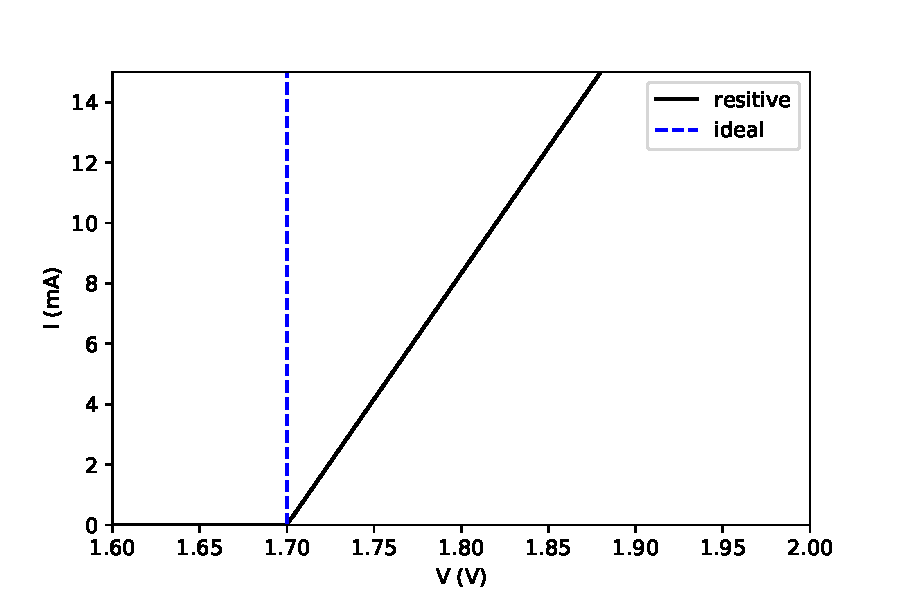
\includegraphics[height=0.3\textheight]{figs/model.pdf} \\
\end{center}
\caption{The LED model for $V_A=1.7~\rm V$ and $R_{\rm LED}=12~\Omega$}
\label{fig:ledmodel}
\end{figure}

\section{Data Collection}

For each of your three reseved LEDs (red, yellow, and green) take a
series of measurements with the applied voltage adjusted so that
$I=5,10,15,20~\rm mA$ and the maximum current (should be just above
20~\rm mA).  You will find that it is difficult to precisely set the
current.  Often when collecting data, you can measure more precisely
than you can set, so always get as close to your target as you can
conveniently reach, and then simply record the actual value.  The
target values simply give you data that is appropriately spaced across
the dynamic range.

Record the color of each LED or simply assign each LED a letter
(A,B,C) for now and determine the color from your data later.
Example instructor data for the red LED is shown in the table.

\begin{table}
\begin{center}
\caption{Instructor data for a red LED.}
\begin{tabular}{lll}
target $I$ (mA) & $I$ (uA) & $V_{\rm D}$ (mV) \\
\hline
5    & 5088  & 1661 \\
10   & 10948 & 1705 \\
15   & 16031 & 1730 \\
20   & 21749 & 1759 \\
MAX  & 25415 & 1779 \\
\end{tabular}
\end{center}
\end{table}

\begin{table}[htbp]
\begin{center}
\caption{LEDs used in this experiment.}
\begin{tabular}{lll}
color & part no. & $\lambda$ (nm) \\
green & LTL-4238 & 565 \\  
yellow & LTL-4256N & 587 \\ 
red & LTL-4268-H3 & 620 \\ 
\end{tabular}
\end{center}
\end{table}

\section{Analysis}

\begin{figure}[htbp]
\begin{center}
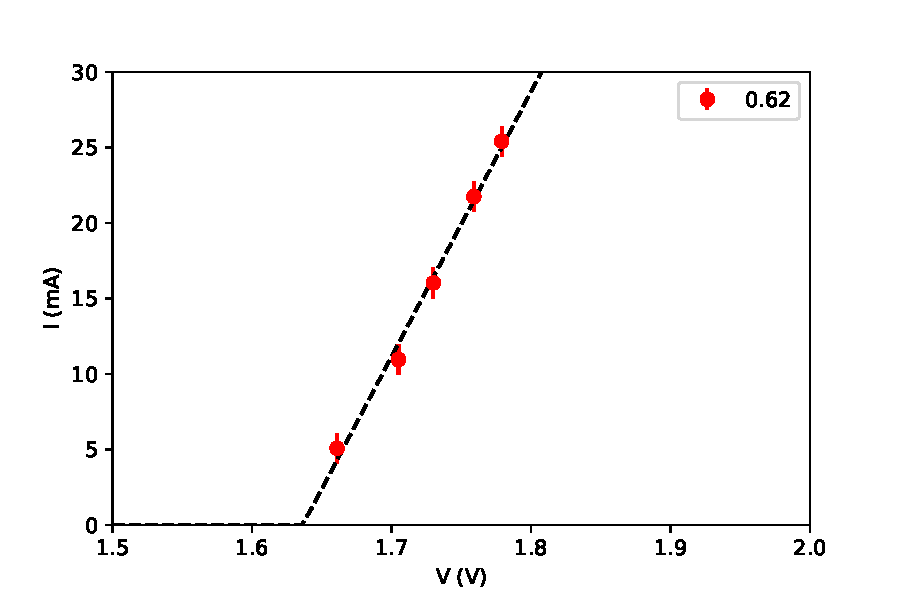
\includegraphics[width=0.45\textwidth]{figs/instructor_red.pdf} \\
\end{center}
\caption{Instructor fit for the red LED.}
\label{fig:redfit}
\end{figure}

The V-I response for a red diode as measured by the instructor is
plotted in Fig~\ref{fig:redfit}.  Notice that at these currents the VI
response is linear, indicating that it is dominated by internal
resistance of the diode, and a simple linear fit will suffice to
determine the activation voltage as the intercept with the voltage
axis.  An example fit for the instructor data is shown in
Fig.~\ref{fig:redfit}.  You can assume the uncertainty on each current
measurement is 1 mA.  For each LED, fit the $V$ versus $I$ data to a
linear function, determine the best fit resistance and activation
voltage, and the uncertainty from the fit.  The red LED will have the
lowest activation energy, and the green LED the highest.

\begin{figure}[htbp]
\begin{center}
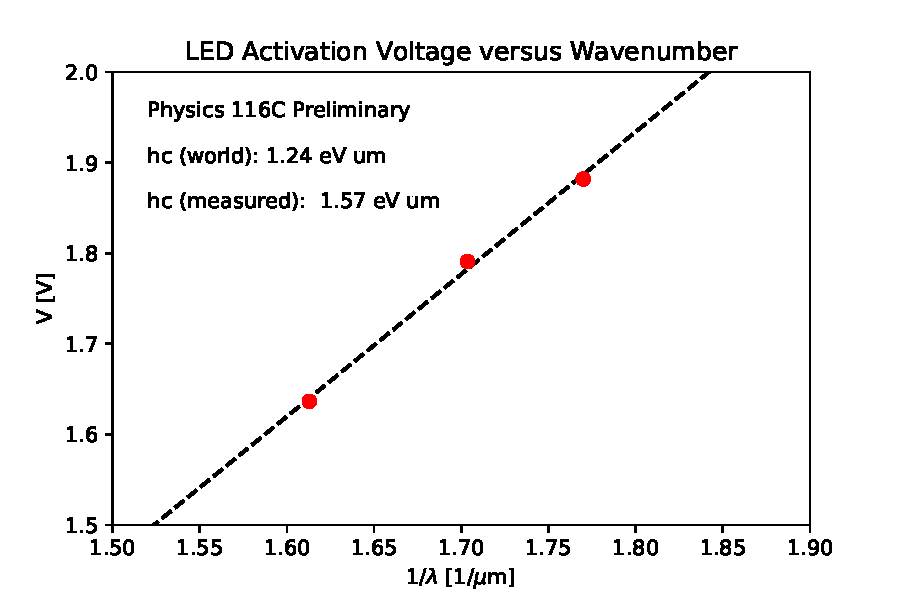
\includegraphics[width=0.45\textwidth]{figs/instructor_planck.pdf} 
\end{center}
\caption{Instructor plot for determination of $hc$.}
\label{fig:planckfit}
\end{figure}


Using the best-fit values of $V_A$ determined from the previous plots,
plot $V_A$ of each diode versus $1/\lambda$, using the wavelengths
determined from the device specs.  Determine the slope ($hc/e$) and
its uncertainty from a linear fit.  The instructor plot is shown in
Fig.~\ref{fig:planckfit}.  Recall that $1~\rm eV$ is the change in
potential energy of one electron passing through $1~\rm V$ of
potential energy, allowing you to conveniently convert the slope in
$\rm V \mu m$ to $\rm eV \mu m$ for comparison with the established
value $hc = 1.240~\rm eV \mu m$.  This measurement is dominated by
systematic effects, notably our assumption that the constant $\phi$ is
common to all devices, which I estimate to be about $20\%$.

\section{Design Improvements}

For fun and extra credit, you can automate the data taking process.
Instead of using the potentiometer output as the adjustable voltage
level, use PWM output at digital pin 5, filtered through the on-device
$RC$ filter, as in the function generator and digital scope exercise.
This will give you digital control of the applied voltage level, which
you can use to automatically scan the VI curve for the
device-under-test.

\end{document}








